\section{Convexité: ensembles et fonctions}\label{subsec:ss_1}

% ----- Consignes exo 1 ----- %
\begin{td-exo}[Convexité]\, % 1 
	\begin{enumerate}
		\item Soit une famille (éventuellement infinie) d'inégalités linéaires
		\(a_i^T x \leq b_i,i\in I\). Soit \(C\) son ensemble de solutions.
		Montrer que \(C\) est convexe.

		\item Montrer que la boule fermée \(\mathsf{B}(a,r)\) est convexe
		pour tout \(a\in\bb R^n\) et \(r\in \bb R^+\).

		\item Soit \(S\subseteq\bb R^n\) et soit \(W\) l'ensemble de toutes les
		combinaisons convexes de points de \(S\). Montrer que \(W\) est convexe.

		\item Soit \(C\) un convexe. Montrer que 
		\begin{equation*}
			\bigcup_{0\leq\lambda\leq 1}\lambda C
		\end{equation*}
		est convexe.

		\item Une matrice \(A=(a_{ij})\) de dimension \(n\times n\) est bistochastique si 
		elle satisfait
		\begin{equation*}
			\begin{aligned}
				\forall i\in\{1,\ldots,n\}, & \sum_{j=1}^n a_{ij} = 1, \\
				\forall j\in\{1,\ldots,n\}, & \sum_{i=1}^n a_{ij} = 1, \\
				\forall (i,j)\in{\{1,\ldots,n\}}^2, & a_{ij}\geq 0.
			\end{aligned}
		\end{equation*}
		Une matrice de permutation \(P\) est une matrice bistochastique à valeurs 
		entières, c'est-à-dire que dans chaque ligne de \(P\) il y a un et un seul élément égal à 1,
		et les autres sont nuls. De même pour chaque colonne.
		\begin{enumerate}
			\item Montrer que pour toute matrice bistochastique \(A\), il existe
			une matrice de permutation \(P\) de même dimension telle que \(p_{ij}=0\)
			si \(a_{ij}=0\).

			\item Est-ce qu'une combinaison convexe de matrices de permutation est 
			une matrice bistochastique?

			\item Montrer que toute matrice bistochastique \(A\) est une combinaison convexe
			de matrices de permutation.

			\item Trouver la combinaison convexe pour la matrice \(A\) suivante:
			\begin{equation*}
				A = \begin{pmatrix}
					0.15 & 0.37 & 0 & 0.48 \\
					0.02 & 0.15 & 0.67 & 0.16 \\
					0.46 & 0.02 & 0.16 & 0.36 \\
					0.37 & 0.46 & 0.17 & 0
				\end{pmatrix}.
			\end{equation*}
		\end{enumerate}

		\item Soient maintenant \(C_1\) et \(C_2\) deux convexes disjoints et
		\begin{equation*}
			D_1 = \bigcup_{0\leq\lambda\leq 1}\lambda C_1, \quad i=1,2.
		\end{equation*}
		Montrer que l'un des deux convexes \(C_1\cap D_2\) ou \(C_2\cap D_1\) est vide.
	\end{enumerate}
\end{td-exo}

% ----- Solutions exo 1 ----- %
\iftoggle{showsolutions}{
	\begin{td-sol}[]\ %
		A remplir %TODO solve exercise 1
	\end{td-sol}
}{}


% ----- Consignes exo 2 ----- %
\begin{td-exo}[Combinaison convexe]\, % 2
	\begin{enumerate}
		\item Rappeler la définition d'une combinaison convexe.
		\item Est-ce que le point \(A\) de coordonnées \((1,1,1)\) est une combinaison convexe
		des points \((2,2,0), (0,0,3), (0,0,0)\)?
		\item Déterminer si le point de coordonnées \((0,7)\) est une combinaison convexe
		des points \((3,6),(-6,9),(2,1),(-1,1)\).
		\item Déterminer graphiquement si le point de coordonnées \((1,2)\) est une combinaison
		convexe des points \((1,1)\) et \((2,-1)\).
	\end{enumerate}
\end{td-exo}

% ----- Solutions exo 2 ----- %
\iftoggle{showsolutions}{
	\begin{td-sol}[]\ %
		\begin{enumerate}
			\item Une combinaison convexe de points \(x_1, x_2, \ldots, x_k\) est une combinaison
			\begin{equation*}
				\sum_{i=1}^k \lambda_i x_i
			\end{equation*}
			avec \(\lambda_i \geq 0\) et \(\sum_{i=1}^k \lambda_i = 1\).

			\item On cherche \(\lambda_1, \lambda_2, \lambda_3 \geq 0\) tels que
			\begin{equation*}
				\lambda_1 (2,2,0) + \lambda_2 (0,0,3) + \lambda_3 (0,0,0) = (1,1,1).
			\end{equation*}
			Ici on voit que \((\lambda1, \lambda_2, \lambda_3) = (0.5, 1/3, 0)\) est une solution.

			\item On cherche \(\lambda_1, \lambda_2, \lambda_3, \lambda_4 \geq 0\) tels que
			\begin{equation*}
				\lambda_1 (3,6) + \lambda_2 (-6,9) + \lambda_3 (2,1) + \lambda_4 (-1,1) = (0,7).
			\end{equation*}
			Cela revient à résoudre le système suivant:
			\begin{equation*}
				\begin{cases}
					3\lambda_1 - 6\lambda_2 + 2\lambda_3 - \lambda_4 = 0 \\
					6\lambda_1 + 9\lambda_2 + \lambda_3 + \lambda_4 = 7 \\
					\lambda_1 + \lambda_2 + \lambda_3 + \lambda_4 = 1
				\end{cases}
			\end{equation*}
			En résolvant on obtient la famille de solutions:
			\begin{equation*}
				\lambda_1 = \frac t2 + \frac 23,\quad
				\lambda_2 = \frac 13 + \frac {5t}{16},\quad
				\lambda_3 = \frac{-19t}{16},\quad
				\lambda_4 = t
			\end{equation*}
			avec \(t\in\bb R\). En imposant \(\lambda_i \geq 0\) on trouve \(t=0\) et donc
			\((\lambda_1, \lambda_2, \lambda_3, \lambda_4) = (2/3, 1/3, 0, 0)\).

			\item Graphiquement, on voit que le point \((1,2)\) n'est pas sur le segment
			entre les points \((1,1)\) et \((2,-1)\). Donc ce n'est pas une combinaison convexe:

			\begin{center}
				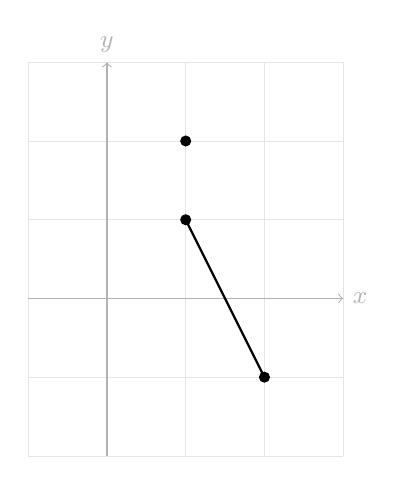
\begin{tikzpicture}[scale=1, font=\small]
					% coordinates
					\coordinate (A) at (1,1);
					\coordinate (B) at (2,-1);
					\coordinate (P) at (1,2);

					% light grid
					\draw[step=1cm, very thin, gray!20] (-1,-2) grid (3,3);

					% axes
					\draw[->, thin, gray!60] (-1,0) -- (3,0) node[right] {\(x\)};
					\draw[->, thin, gray!60] (0,-2) -- (0,3) node[above] {\(y\)};

					% segment AB
					\draw[thick] (A) -- (B) node[midway, below right=1pt] {};

					% points
					\fill (A) circle (2pt) node[below left=2pt] {};
					\fill (B) circle (2pt) node[below right=2pt] {};
					\fill (P) circle (2pt) node[above left=2pt] {};
				\end{tikzpicture}\,
			\end{center}
		\end{enumerate}
	\end{td-sol}
}{}


% ----- Consignes exo 3 ----- %
\begin{td-exo}[Ensembles convexe]\,\\ % 3
	Montrer qu'étant donné un sous-ensemble convexe \(C\) et deux réels positifs \(\alpha\) et \(\beta\)
	alors on a
	\begin{equation*}
		\alpha C + \beta C = (\alpha + \beta) C.
	\end{equation*}
\end{td-exo}

% ----- Solutions exo 3 ----- %
\iftoggle{showsolutions}{
	\begin{td-sol}[]\ %
		Commencons par montrer l'inclusion \(\left(\alpha + \beta\right) C \subset \alpha C + \beta C\).

		Soit \(x \in \left(\alpha + \beta\right) C\). Alors, il existe \(x_0\in C\) tel que
		\begin{equation*}
			x = \left(\alpha + \beta\right) x_0 = \alpha x_0 + \beta x_0.
		\end{equation*}
		
		Donc \(x \in \alpha C + \beta C\).

		Montrons maintenant l'inclusion \(\alpha C + \beta C \subset \left(\alpha + \beta\right) C\).

		Soit \(x \in \alpha C + \beta C\). Alors, il existe \(x_1, x_2 \in C\) tels que
		\begin{equation*}
			x = \alpha x_1 + \beta x_2 = \left(\alpha + \beta\right) \left(\frac{\alpha}{\alpha + \beta} x_1 + \frac{\beta}{\alpha + \beta} x_2\right).
		\end{equation*}
	\end{td-sol}
}{}


% ----- Consignes exo 4 ----- %
\begin{td-exo}[Ensembles convexes]\,\\ % 4
	Soit \(S\sub\bb R^n\) vérifiant la propriété de \defemph{demi-somme} suivante:
	\begin{equation*}
		\forall x,y \in S,\quad \frac{x+y}{2} \in S.
	\end{equation*}

	\begin{enumerate}
		\item \(S\) est-il convexe?

		\item Même question si on suppose que \(S\) est fermé.
	\end{enumerate}
\end{td-exo}

% ----- Solutions exo 4 ----- %
\iftoggle{showsolutions}{
	\begin{td-sol}[]\ %
		\begin{enumerate}
			\item Non. Par exemple, le sous-ensemble \(S\) suivant:
			\begin{equation*}
				S = \left\{ x \in \ff{0,1} \mid x = \sum_{i=I} \frac{1}{2^i} \right\} = \left\{ 0, \frac{1}{2}, \frac{1}{4}, \frac{3}{4}, \ldots \right\}
			\end{equation*}
			vérifie la propriété de demi-somme mais n'est pas convexe, car par exemple \(\sqrt{2}/2 \in \ff{0,1} \notin S\).
		\end{enumerate}
	\end{td-sol}
}{}


% ----- Consignes exo 5 ----- %
\begin{td-exo}[Ensembles convexes]\,\\ % 5
	Lesquels de ces ensembles sont convexes?
	\begin{enumerate}
		\item \(S=\left\{(x_1,x_2)\ \mid\ 3x_1^2 + 2x_2^2 \leq 12\right\}\),
		\item \(S=\left\{(x_1,x_2)\ \mid\ x_1 \geq 3, x_1 \leq 5\right\}\).
	\end{enumerate}
\end{td-exo}

% ----- Solutions exo 5 ----- %
\iftoggle{showsolutions}{
	\begin{td-sol}[]\ %
		A remplir %TODO solve exercise 5
	\end{td-sol}
}{}


% ----- Consignes exo 6 ----- %
\begin{td-exo}[Ensembles convexes]\ % 6
	\begin{enumerate}
		\item Soit \(C\) un convexe. Montrer que \(x\in C\) est un point extrême de \(C\)
		si et seulement si \(C\setminus\{x\}\) est convexe.

		\item A-t-on une caractérisation similaire pour une face de \(C\)?

		\item On considère dans \(\bb R^n\) les deux boules suivantes:
		\begin{itemize}
			\item \(\mathsf{B}_1=\{x = (x_1,\ldots,x_n)\in \bb R^n\ \mid\ \sum_{i=1}^\infty \n{x_i} \leq 1\}\)
			\item \(\mathsf{B}_\infty = \{x = (x_1,\ldots,x_n)\in \bb R^n\ \mid\ \max_{1\leq i\leq n} \n{x_i} \leq 1\}\)
		\end{itemize}
		Quels sont les points extrêmes de \(\mathsf{B}_1\) et \(\mathsf{B}_\infty\)?
	\end{enumerate}
\end{td-exo}

% ----- Solutions exo 6 ----- %
\iftoggle{showsolutions}{
	\begin{td-sol}[]\ %
		\begin{enumerate}
			\item Commencons par le sens direct:\\
			Soit \(x\in C\) un point extrême de \(C\). Montrons que \(C\setminus\{x\}\) est convexe.

			Soit \(y,z \in C\setminus\{x\}\) et \(\lambda \in \ff{0,1}\). Alors
			\begin{equation*}
				\lambda y + (1-\lambda) z \in C.
			\end{equation*}
			car \(C\) est convexe. Supposons par l'absurde que \(\lambda y + (1-\lambda) z = x\). 
			Alors \(x\) est une combinaison convexe de \(y\) et \(z\) avec \(\lambda \in \ff{0,1}\).
			Cela contredit le fait que \(x\) est un point extrême de \(C\). Donc la
			combinaison convexe \(\lambda y + (1-\lambda) z\) est dans \(C\setminus\{x\}\).
			Donc \(C\setminus\{x\}\) est convexe.

			Montrons maintenant le sens réciproque:\\
			Soit \(x\in C\) tel que \(C\setminus\{x\}\) est convexe. Montrons que \(x\) est un point extrême de \(C\).

			Supposons par l'absurde que \(x\) n'est pas un point extrême de \(C\). Alors, il existe \(y,z \in C\) et \(\lambda \in \oo{0,1}\) tels que
			\begin{equation*}
				x = \lambda y + (1-\lambda) z.
			\end{equation*}
			Comme \(y,z \in C\) et \(x\) est une combinaison convexe de \(y\) et \(z\), on a forcément \(y \neq x\) et \(z \neq x\).
			Donc \(y,z \in C\setminus\{x\}\). Comme \(C\setminus\{x\}\) est convexe, on a
			\begin{equation*}
				x = \lambda y + (1-\lambda) z \in C\setminus\{x\}.
			\end{equation*}
			C'est une contradiction. Donc \(x\) est un point extrême de \(C\).
		\end{enumerate}
	\end{td-sol}
}{}


% ----- Consignes exo 7 ----- %
\begin{td-exo}[Fonction convexe]\ % 7
	\begin{enumerate}
		\item Est-ce qu'une combinaison linéaire à coefficients positifs de fonctions convexes est convexe?

		\item Est-ce que le produit de deux fonctions convexes est convexe?

		\item Si \(f_1\) et \(f_2\) sont deux fonctions convexes, est-ce que \(\max\left(f_1,f_2\right)\) est convexe?

		\item Montrer que la fonction \(f\ \colon\ x\mapsto x^2\) est une fonction convexe sur \(\bb R\).
	\end{enumerate}
\end{td-exo}

% ----- Solutions exo 7 ----- %
\iftoggle{showsolutions}{
	\begin{td-sol}[]\ %
		\begin{enumerate}
			\item Oui. On pose \(g(x) = \sum_{i\in I} \alpha_i f_i(x)\). Alors
			\begin{equation*}
				\begin{aligned}
					g(\lambda x + (1-\lambda) y) 
					& = \sum_{i\in I} \alpha_i f_i(\lambda x + (1-\lambda) y) \\
					& \leq \sum_{i\in I} \alpha_i \left(\lambda f_i(x) + (1-\lambda) f_i(y)\right) \\
					& = \lambda g(x) + (1-\lambda) g(y).
				\end{aligned}
			\end{equation*}

			\item Non. Par exemple, \(f_1(x) = x\) et \(f_2(x) = x^2\) sont convexes mais \(f_1(x) f_2(x) = x^3\) n'est pas convexe.

			\item Oui. On pose \(g(x) = \max\left(f_1(x), f_2(x)\right)\). Alors
			\begin{equation*}
				\begin{aligned}
					g(\lambda x + (1-\lambda) y) 
					& = \max\left(f_1(\lambda x + (1-\lambda) y), f_2(\lambda x + (1-\lambda) y)\right) \\
					& \leq \max\left(\lambda f_1(x) + (1-\lambda) f_1(y), \lambda f_2(x) + (1-\lambda) f_2(y)\right) \\
					& \leq \lambda \max\left(f_1(x), f_2(x)\right) + (1-\lambda) \max\left(f_1(y), f_2(y)\right) \\
					& = \lambda g(x) + (1-\lambda) g(y).
				\end{aligned}
			\end{equation*}

			\item Soit \(x,y \in \bb R\) et \(\lambda \in [0,1]\). Alors
			\begin{equation*}
				\begin{aligned}
					f(\lambda x + (1-\lambda) y) 
					& = {(\lambda x + (1-\lambda) y)}^2 \\
					& = \lambda^2 x^2 + {(1-\lambda)}^2 y^2 + 2\lambda(1-\lambda) xy \\
					& \iff \lambda^2 x^2 + {(1-\lambda)}^2 y^2 + 2\lambda(1-\lambda) xy - \lambda x^2 - (1-\lambda) y^2 \leq 0 \\
					& \iff \lambda (1-\lambda)\left(\frac{\lambda}{1-\lambda} x^2 + \frac{1-\lambda}{\lambda} y^2 + 2xy - \frac{x^2}{1-\lambda} - \frac{y^2}{\lambda}\right) \leq 0 \\
					& \iff \lambda (1-\lambda)\left(-{\left(x - y\right)}^2\right) \leq 0.
				\end{aligned}
			\end{equation*}
			Or tous les termes sont positifs sauf le dernier. Donc l'inégalité est vérifiée.
		\end{enumerate}
	\end{td-sol}
}{}


% ----- Consignes exo 8 ----- %
\begin{td-exo}[Fonction convexe]\,\\% 8
	Soit \(f\ \colon\ \bb R^n \to \bb R\) une fonction continue telle que
	\begin{equation*}
		\forall (x,y) \in \bb R^2, \quad f\left(\frac{x+y}{2}\right) \leq \frac{f(x) + f(y)}{2}.
	\end{equation*}
	Prouver que \(f\) est convexe.\\
	Indication: Montrer par récurrence que sur \(\n\geq 2\), on a
	\begin{equation*}
		\forall (x,y) \in \bb R^2, \forall p\in\{0,1,\ldots,2^n\}, \quad f \left( \frac p{2^n}x + \left(1 - \frac p{2^n}\right)y\right) \leq \frac p{2^n} f(x) + \left(1 - \frac p{2^n}\right) f(y).
	\end{equation*}
\end{td-exo}

% ----- Solutions exo 8 ----- %
\iftoggle{showsolutions}{
	\begin{td-sol}[]\ %
		A remplir %TODO solve exercise 8
	\end{td-sol}
}{}

\section{Divers formulations}

% ----- Consignes exo 9 ----- %
\begin{td-exo}[Reformulation en programme linéaire]\,\\% 9
	Reformuler les problèmes suivants sous forme de programme linéaire.
	\begin{enumerate}
		\item \begin{equation*}
			\begin{cases}
				\min z = 2x_1 + 3 \n{x_2 - 10} \\
				\n{x_1 + 2} + \n {x_2} \leq 5\\
				2x_1 + x_2 \leq 4
			\end{cases}
		\end{equation*}
	\end{enumerate}

	\item Soit un ensemble d'inégalités linéaires 
	\begin{equation*}
		a_i^T x \leq b_i, \quad i=1,\ldots,m,a_i\in\bb R^n,b_i\in\bb R.
	\end{equation*}
	Formuler un modèle (uniquement des contraintes sans fonction objectif) pour lequel un point \(x\in\bb N^n\)
	satisfait au moins \(k\) des \(m\) contraintes (\(k\leq m\)) entiers de plus satisfaite
	\begin{equation*}
		0\leq x_j \leq M,\quad \forall j \in \{1,\ldots,m\}.
	\end{equation*}
\end{td-exo}

% ----- Solutions exo 9 ----- %
\iftoggle{showsolutions}{
	\begin{td-sol}[]\ %
		A remplir %TODO solve exercise 9
	\end{td-sol}
}{}


% ----- Consignes exo 10 ----- %
\begin{td-exo}[Linéarisation de fonctions non linéaires] % 10
	A remplir %TODO write exercise 10
\end{td-exo}

% ----- Solutions exo 10 ----- %
\iftoggle{showsolutions}{
	\begin{td-sol}[]\ %
		A remplir %TODO solve exercise 10
	\end{td-sol}
}{}


% ----- Consignes exo 11 ----- %
\begin{td-exo}[] % 11
	A remplir %TODO write exercise 11
\end{td-exo}

% ----- Solutions exo 11 ----- %
\iftoggle{showsolutions}{
	\begin{td-sol}[]\ %
		A remplir %TODO solve exercise 11
	\end{td-sol}
}{}

% ----- Consignes exo 12 ----- %
\begin{td-exo}[Forme standard et forme canonique]\,\\ % 12
	Dans cet exercice vous devez mettre les programmes suivants sous forme standard et donner
	également la forme matricielle.
	\begin{enumerate}
		\item
		\begin{equation*}
			\begin{cases}
				\max z = x_1 + x_2 \\
				x_1 + 5 x_2 \leq 5 \\
				2x_1 + x_2 \leq 4 \\
				x_1 \geq 0,\quad i=1,2.
			\end{cases}
		\end{equation*}

		\item
		\begin{equation*}
			\begin{cases}
				\max z = 80 x_1 + 60 x_2 \\
				0.2x_1 + 0.32 x_2 \leq 0.25\\
				x_1 + x_2 = 1 \\
				x_1 \geq 0,\quad i=1,2.
			\end{cases}
		\end{equation*}

		\item Réécrire le programme précédent dans le cas où la fonction objectif
		est la minimisation.

		\item
		\begin{equation*}
			\begin{cases}
				\max z = 5x_1 + 2x_2 \\
				6x_1 + x_2 \geq 6 \\
				4x_1 + 3x_2  \geq 12 \\
				x_1 + 2x_2 \geq 4 \\
				x_1 \geq 0,\quad i=1,2.
			\end{cases}
		\end{equation*}
	\end{enumerate}
\end{td-exo}

% ----- Solutions exo 12 ----- %
\iftoggle{showsolutions}{
	\begin{td-sol}[]\ %
		\begin{enumerate}
			\item La forme standard est
			\begin{equation*}
				\begin{cases}
					\max z = x_1 + x_2 + 0\cdot x_3 + 0\cdot x_4 \\
					x_1 + 5 x_2 + x_3 = 5 \\
					2x_1 + x_2 + x_4 = 4 \\
					x_1, x_2, x_3, x_4 \geq 0.
				\end{cases}
			\end{equation*}
			La forme matricielle est
			\begin{equation*}
				\begin{cases}
					\max z = \begin{pmatrix} 1 & 1 & 0 & 0 \end{pmatrix} \begin{pmatrix} x_1 \\ x_2 \\ x_3 \\ x_4 \end{pmatrix} \\
					\begin{pmatrix}
						1 & 5 & 1 & 0 \\
						2 & 1 & 0 & 1
					\end{pmatrix}
					\begin{pmatrix} x_1 \\ x_2 \\ x_3 \\ x_4 \end{pmatrix}
					=
					\begin{pmatrix} 5 \\ 4 \end{pmatrix}, \quad
					\begin{pmatrix} x_1 \\ x_2 \\ x_3 \\ x_4 \end{pmatrix} \geq 0.
				\end{cases}
			\end{equation*}

			\item La forme standard est
			\begin{equation*}
				\begin{cases}
					\max z = 80 x_1 + 60 x_2 + 0\cdot x_3 - M \cdot x_4\\
					0.2x_1 + 0.32 x_2 + x_3 = 0.25\\
					x_1 + x_2 + x_4 = 1 \\
					x_1, x_2, x_3, x_4 \geq 0.
				\end{cases}
			\end{equation*}
			La forme matricielle est
			\begin{equation*}
				\begin{cases}
					\max z = \begin{pmatrix} 80 & 60 & 0 & -M \end{pmatrix} \begin{pmatrix} x_1 \\ x_2 \\ x_3 \\ x_4 \end{pmatrix} \\
					\begin{pmatrix}
						0.2 & 0.32 & 1 & 0 \\
						1 & 1 & 0 & 1
					\end{pmatrix}
					\begin{pmatrix} x_1 \\ x_2 \\ x_3 \\ x_4 \end{pmatrix}
					=
					\begin{pmatrix} 0.25 \\ 1 \end{pmatrix},\quad
					\begin{pmatrix} x_1 \\ x_2 \\ x_3 \\ x_4 \end{pmatrix} \geq 0.
				\end{cases}
			\end{equation*}

			\item La forme standard est
			\begin{equation*}
				\begin{cases}
					\min z = -80 x_1 - 60 x_2 + 0\cdot x_3 + M \cdot x_4\\
					0.2x_1 + 0.32 x_2 + x_3 = 0.25\\
					x_1 + x_2 + x_4 = 1 \\
					x_1, x_2, x_3, x_4 \geq 0.
				\end{cases}
			\end{equation*}
			La forme matricielle est
			\begin{equation*}
				\begin{cases}
					\min z = \begin{pmatrix} -80 & -60 & 0 & M \end{pmatrix} \begin{pmatrix} x_1 \\ x_2 \\ x_3 \\ x_4 \end{pmatrix} \\
					\begin{pmatrix}
						0.2 & 0.32 & 1 & 0 \\
						1 & 1 & 0 & 1
					\end{pmatrix}
					\begin{pmatrix} x_1 \\ x_2 \\ x_3 \\ x_4 \end{pmatrix}
					=
					\begin{pmatrix} 0.25 \\ 1 \end{pmatrix}, \quad
					\begin{pmatrix} x_1 \\ x_2 \\ x_3 \\ x_4 \end{pmatrix} \geq 0.
				\end{cases}
			\end{equation*}

			\item La forme standard est
			\begin{equation*}
				\begin{cases}
					\max z = 5x_1 + 2x_2 + 0\cdot x_3 + 0\cdot x_4 + 0\cdot x_5 + M\cdot (x_6 + x_7 + x_8)\\
					6x_1 + x_2 - x_3 + x_6= 6 \\
					4x_1 + 3x_2 - x_4 + x_7 = 12 \\
					x_1 + 2x_2 - x_5 + x_8 = 4 \\
					x_1, x_2, x_3, x_4, x_5, x_6, x_7, x_8 \geq 0.
				\end{cases}
			\end{equation*}
			La forme matricielle est
			\begin{equation*}
				\begin{cases}
					\max z = \begin{pmatrix} 5 & 2 & 0 & 0 & 0 & M & M & M \end{pmatrix} \begin{pmatrix} x_1 \\ x_2 \\ x_3 \\ x_4 \\ x_5 \\ x_6 \\ x_7 \\ x_8 \end{pmatrix} \\
					\begin{pmatrix}
						6 & 1 & -1 & 0 & 0 & 1 & 0 & 0 \\
						4 & 3 & 0 & -1 & 0 & 0 & 1 & 0 \\
						1 & 2 & 0 & 0 & -1 & 0 & 0 & 1
					\end{pmatrix}
					\begin{pmatrix} x_1 \\ x_2 \\ x_3 \\ x_4 \\ x_5 \\ x_6 \\ x_7 \\ x_8 \end{pmatrix}
					=
					\begin{pmatrix} 6 \\ 12 \\ 4 \end{pmatrix}, \quad
					\begin{pmatrix} x_1 \\ x_2 \\ x_3 \\ x_4 \\ x_5 \\ x_6 \\ x_7 \\ x_8 \end{pmatrix} \geq 0.
				\end{cases}
			\end{equation*}
		\end{enumerate}
	\end{td-sol}
}{}


% ----- Consignes exo 13 ----- %
\begin{td-exo}[]\,\\ % 13
	Nous considérons les programmes linéaires avec des variables \(x_1\in\{0, u_j\}\).
	Montrer que nous pouvons nous ramener à un programme linéaire en nombres entiers.
	Appliquez-le au problème suivant:
	\begin{equation*}
		\begin{cases}
			\max z = 18x_1 + 3x_2 + 9x_3 \\
			2x_1 + x_2 + 7x_3 \leq 150 \\
			x_1 \in \{0, 60\} \\
			x_2 \in \{0, 30\} \\
			x_3 \in \{0, 20\}.
		\end{cases}
	\end{equation*}
\end{td-exo}

% ----- Solutions exo 13 ----- %
\iftoggle{showsolutions}{
	\begin{td-sol}[]\ %
		On remplace chaque variable \(x_j\) par une variable \(y_j\) telle que \(x_j = u_j y_j\)
		et \(y_j \in \{0,1\}\). Le programme devient
		\begin{equation*}
			\begin{cases}
				\max z = 18\cdot 60 y_1 + 3\cdot 30 y_2 + 9\cdot 20 y_3 \\
				2\cdot 60 y_1 + 30 y_2 + 7\cdot 20 y_3 \leq 150 \\
				y_1, y_2, y_3 \in \{0,1\}.
			\end{cases}
		\end{equation*}
		Cela revient à résoudre le programme linéaire en nombres entiers suivant:
		\begin{equation*}
			\begin{cases}
				\max z = 1080 y_1 + 90 y_2 + 180 y_3 \\
				120 y_1 + 30 y_2 + 140 y_3 \leq 150 \\
				y_1, y_2, y_3 \in \{0,1\}.
			\end{cases}
		\end{equation*}
	\end{td-sol}
}{}


% ----- Consignes exo 14 ----- %
\begin{td-exo}[Points extrêmes]\,\\ % 14
	On considère le polyèdre \(S\) de \(\bb R^3\) défini par les conditions suivantes:
	\begin{equation*}
		\begin{cases}
			x_1 + x_3 + x_5 = 2\\
			2x_2 + x_3 + x_4 = 4\\
			x_1 + x_2 + x_4 + 2x_5 = 3\\
			x_i \geq 0, \quad i=1,\ldots,5.
		\end{cases}
	\end{equation*}
	\begin{enumerate}
		\item Le point \(x*=(1,1,1,1,0)\) est-il un point extrême? Pourquoi?

		\item Les points suivants sont-ils des points extrêmes? Dégénérés?
		\begin{itemize}
			\item \(x_1 = (0,-1,2,4,0)\),
			\item \(x_2 = (0.5,0,1.5,2.5,0)\),
			\item \(x_3 = (2,3,0,-2,0)\),
			\item \(x_4 = (\frac43,\frac53,\frac23,0,0)\).
		\end{itemize}
	\end{enumerate}
\end{td-exo}

% ----- Solutions exo 14 ----- %
\iftoggle{showsolutions}{
	\begin{td-sol}[]\ %
		\begin{enumerate}
			\item On commence par vérifier que \(x*\) respecte les contraintes: %TODO

			On constate qu'il vérifie bien les contraintes, mais on sait qu'il n'y a
			que 3 variables en base. Or, \(x*\) en a 4 de non nulles. Donc, \(x*\) n'est pas un point extrême.

			\item On commence par vérifier que les points respectent les contraintes:
			\begin{itemize}
				\item \(x_1\) ne respecte pas les contraintes car \(x_2 < 0\).
				\item \(x_2\) respecte les contraintes et a 3 variables en base. Donc, \(x_2\) est un point extrême non dégénéré.
				\item \(x_3\) ne respecte pas les contraintes car \(x_4 < 0\).
				\item \(x_4\) respecte les contraintes et a 3 variables en base. Donc, \(x_4\) est un point extrême non dégénéré.
			\end{itemize}
			On rappelle qu'un point est dégénéré s'il a plus de \(m\) variables nulles où \(m\) est le nombre de variables originelles.
		\end{enumerate}
	\end{td-sol}
}{}


% ----- Consignes exo 15 ----- %
\begin{td-exo}[Points extrêmes et solutions]\,\\ % 15
	Soit le polyèdre \(P = \{x \in \bb R^3 \mid Ax \leq b\}\) avec
	\begin{equation*}
		A = \begin{pmatrix}
			2, 3, 6 \\
			-1, 0, 0 \\
			0, -1, 0 \\
			0, 0, -1 \\
		\end{pmatrix}, \quad
		b = \begin{pmatrix}
			6, 1, 0, 0
		\end{pmatrix}.
	\end{equation*}
	On supposera que le polyèdre est borné.

\end{td-exo}

% ----- Solutions exo 15 ----- %
\iftoggle{showsolutions}{
	\begin{td-sol}[]\ %
		Pour trouver les points extrêmes, on cherche à résoudre
		tous les arrangements possibles de 3 contraintes parmi les 4.
		On énumère les lignes qu'on choisit comme contraintes comme suit et on les résout dans l'ordre:
		\begin{equation*}
			(1,2,3), (1,2,4), (1,3,4), (2,3,4).
		\end{equation*}
		\begin{itemize}
			\item Pour (1,2,3), on résout:
			\begin{equation*}
				\begin{cases}
					2x_1 + 3x_2 + 6x_3 = 6\\
					-x_1 = 1\\
					-x_2 = 0
				\end{cases}
			\end{equation*}
			et on trouve \(x_1 = (-1, 0, \frac43)\).
			\item Pour (1,2,4), on trouve \(x_2 = (-1, \frac83, 6)\),
			\item Pour (1,3,4), on trouve \(x_3 = (3, 0, 0)\),
			\item Pour (2,3,4), on trouve \(x_4 = (-1, 0, 0)\).	
		\end{itemize}
		Les points extrêmes sont donc \(x_1, x_2, x_3\) et \(x_4\).
		Si on rajoute la contrainte \(x_i \geq 0\), on a seulement \(x_3\) qui reste.
	\end{td-sol}
}{}


% ----- Consignes exo 16 ----- %
\begin{td-exo}[Points extrêmes]\,\\ % 16
	Soit \(C\) le polyèdre convexe fermé de \(\bb R^2\) 
	décrit à l'aide des inégalités suivantes:
	\begin{equation*}
		\mathcal{P}_y =
		\begin{cases}
			x_1 + \frac83 x_2 \leq 4\\
			x_1 + x_2 \leq 2\\
			2x_1 \leq 3\\
			x_1 \geq 0\\
		\end{cases}
	\end{equation*}
	
	\begin{enumerate}
		\item Ecrire \(C\) sous la forme standard.
		\item Quels sont les points extrêmes de \(C\)?
	\end{enumerate}
\end{td-exo}

% ----- Solutions exo 16 ----- %
\iftoggle{showsolutions}{
	\begin{td-sol}[]\ %
		\begin{enumerate}
			\item On introduit les variables d'écart \(x_3, x_4, x_5\) pour obtenir la forme standard:
			\begin{equation*}
				\begin{cases}
					x_1 + \frac83 x_2 + x_3 = 4\\
					x_1 + x_2 + x_4 = 2\\
					2x_1 + x_5 = 3\\
					x_i \geq 0, \quad i=1,\ldots,5.
				\end{cases}
			\end{equation*}

			\item On écrit le problème matriciellement:
			\begin{equation*}
				\begin{cases}
					\begin{pmatrix}
						1 & \frac83 & 1 & 0 & 0 \\
						1 & 1 & 0 & 1 & 0 \\
						2 & 0 & 0 & 0 & 1
					\end{pmatrix}
				\end{cases}
			\end{equation*}
			On choisit ensuite 3 contraintes parmi les 5 et on résout les systèmes linéaires associés:
			\begin{itemize}
				\item Pour (3,4,5), on trouve \(x_1 = (0, 0, 4,2,3)\),
				\item Pour (1,2,3), on trouve \(x_2 = (\frac32, \frac12, \frac76, 0, 0)\),
			\end{itemize}
			et ainsi de suite. 
		\end{enumerate}
	\end{td-sol}
}{}


% ----- Consignes exo 17 ----- %
\begin{td-exo}[] % 17
	Soient: \(P = \{x\in\bb R^n: Ax\geq b, x\geq0\}\) et \(Q = \{(x,y)\in\bb R^n\times\bb R^n: Ax-y = b,x\geq0,y\geq0\}\).
	\begin{enumerate}
		\item Montrer que si \(x\) est un point extreme de \(P\), alors
		\(x, Ax-b\) est un point extrême de \(Q\).

		\item Montrer que si \((x,y)\) est un point extrême de \(Q\), alors \(x\) est un point extrême de \(P\).
	\end{enumerate}
\end{td-exo}

% ----- Solutions exo 17 ----- %
\iftoggle{showsolutions}{
	\begin{td-sol}[]\ %
		\begin{enumerate}
			\item Supposons que \(x\) est un point extrême de \(P\). Montrons que \((x,Ax-b)\) est un point extrême de \(Q\).

			Si \((x, Ax-b)\) n'est pas un point extrême de \(Q\), alors il existe \(x_1, x_2 \in Q\) 
			tels que
			\begin{equation*}
				(x, Ax-b) = \frac{x_1, y_1 + x_2, y_2}{2}
			\end{equation*}
			De plus
			\begin{equation*}
				\begin{cases}
					Ax_1 - y_1 = b \implies & Ax_1 \geq b \\
					Ax_2 - y_2 = b \implies & Ax_2 \geq b
				\end{cases}
			\end{equation*}
			Donc \(x_1, x_2 \in P\) et donc \(x = \frac{x_1 + x_2}{2}\in P\).
			Cela contredit le fait que \(x\) est un point extrême de \(P\). Donc \((x,Ax-b)\) est un point extrême de \(Q\).

			\item Supposons que \(x\) n'est pas un point extreme de \(P\). Alors il existe
			\(x_1, x_2 \in P\) tels que \(x = \frac{x_1 + x_2}{2}\). Alors

			\begin{equation*}
				\begin{aligned}
					y
					&= Ax-b\\
					&= A\frac{x_1}2 + A\frac{x_2}2 - b\\
					&= A\frac{x_1}2 + A\frac{x_2}2 - \frac{b}2 - \frac{b}2\\
					&= \frac12\left(Ax_1 - b\right) + \frac12\left(Ax_2 - b\right)\\
					&= \frac{y_1 + y_2}{2}
				\end{aligned}
			\end{equation*}
			d'où
			\begin{equation*}
				\begin{aligned}
					(x,y) = \frac12\left(x_1, y_1\right) + \frac12\left(x_2, y_2\right)
				\end{aligned}
			\end{equation*}
			et donc \((x,y)\) n'est pas un point extrême de \(Q\).
		\end{enumerate}
	\end{td-sol}
}{}


% ----- Consignes exo 18 ----- %
\begin{td-exo}[] % 18
	A remplir %TODO write exercise 18
\end{td-exo}

% ----- Solutions exo 18 ----- %
\iftoggle{showsolutions}{
	\begin{td-sol}[]\ %
		A remplir %TODO solve exercise 18
	\end{td-sol}
}{}


% ----- Consignes exo 18 ----- %
\begin{td-exo}[] % 18
	A remplir %TODO write exercise 18
\end{td-exo}

% ----- Solutions exo 18 ----- %
\iftoggle{showsolutions}{
	\begin{td-sol}[]\ %
		A remplir %TODO solve exercise 18
	\end{td-sol}
}{}


% ----- Consignes exo 18 ----- %
\begin{td-exo}[] % 18
	A remplir %TODO write exercise 18
\end{td-exo}

% ----- Solutions exo 18 ----- %
\iftoggle{showsolutions}{
	\begin{td-sol}[]\ %
		A remplir %TODO solve exercise 18
	\end{td-sol}
}{}


% ----- Consignes exo 18 ----- %
\begin{td-exo}[] % 18
	A remplir %TODO write exercise 18
\end{td-exo}

% ----- Solutions exo 18 ----- %
\iftoggle{showsolutions}{
	\begin{td-sol}[]\ %
		A remplir %TODO solve exercise 18
	\end{td-sol}
}{}


% ----- Consignes exo 18 ----- %
\begin{td-exo}[] % 18
	A remplir %TODO write exercise 18
\end{td-exo}

% ----- Solutions exo 18 ----- %
\iftoggle{showsolutions}{
	\begin{td-sol}[]\ %
		A remplir %TODO solve exercise 18
	\end{td-sol}
}{}


% ----- Consignes exo 18 ----- %
\begin{td-exo}[] % 18
	A remplir %TODO write exercise 18
\end{td-exo}

% ----- Solutions exo 18 ----- %
\iftoggle{showsolutions}{
	\begin{td-sol}[]\ %
		A remplir %TODO solve exercise 18
	\end{td-sol}
}{}


% ----- Consignes exo 18 ----- %
\begin{td-exo}[] % 18
	A remplir %TODO write exercise 18
\end{td-exo}

% ----- Solutions exo 18 ----- %
\iftoggle{showsolutions}{
	\begin{td-sol}[]\ %
		A remplir %TODO solve exercise 18
	\end{td-sol}
}{}


% ----- Consignes exo 18 ----- %
\begin{td-exo}[] % 18
	A remplir %TODO write exercise 18
\end{td-exo}

% ----- Solutions exo 18 ----- %
\iftoggle{showsolutions}{
	\begin{td-sol}[]\ %
		A remplir %TODO solve exercise 18
	\end{td-sol}
}{}


% ----- Consignes exo 18 ----- %
\begin{td-exo}[] % 18
	A remplir %TODO write exercise 18
\end{td-exo}

% ----- Solutions exo 18 ----- %
\iftoggle{showsolutions}{
	\begin{td-sol}[]\ %
		A remplir %TODO solve exercise 18
	\end{td-sol}
}{}


% ----- Consignes exo 18 ----- %
\begin{td-exo}[] % 18
	A remplir %TODO write exercise 18
\end{td-exo}

% ----- Solutions exo 18 ----- %
\iftoggle{showsolutions}{
	\begin{td-sol}[]\ %
		A remplir %TODO solve exercise 18
	\end{td-sol}
}{}


% ----- Consignes exo 18 ----- %
\begin{td-exo}[] % 18
	A remplir %TODO write exercise 18
\end{td-exo}

% ----- Solutions exo 18 ----- %
\iftoggle{showsolutions}{
	\begin{td-sol}[]\ %
		A remplir %TODO solve exercise 18
	\end{td-sol}
}{}


% ----- Consignes exo 29 ----- %
\begin{td-exo}[La méthode du simplexe n'est pas une méthode polynomiale]\,\\ % 29
	Dans cet exercice nous allons montrer que la méthode du simplexe n'est pas une méthode polynomiale.
	Pour cela, nous allons considérer le programme linéaire suivant:
	\begin{equation*}
		(PL_n)=
		\begin{cases}
			\max z = 2^{n-1} x_1 + 2^{n-2} x_2 + \cdots + 2x_{n-1} + x_n \\
			x_1 \leq 5\\
			4x_1 + x_2 \leq 25\\
			8x_1 + 4x_2 + x_3 \leq 125\\
			\ldots\\
			2^n x_1 + 2^{n-1} x_2 + \cdots + 4x_{n-1} + x_n \leq 5^n\\
			x_i \geq 0, \quad i=1,\ldots,n.
		\end{cases}
	\end{equation*}\,
	\begin{enumerate}
		\item Donner la forme standard de \((PL_n)\).
		\item Donner la solution optimale.
		\item Montrer que \(\forall i, x_i\) et \(y_i\) (où \(y_i\) est la variable d'écart associée à la \(i\)-ième
		variable) ne peuvent être en même temps des variables hors base.
		\item Nous allons montrer que \(2^n\) tableaux sont nécessaires pour résoudre ce problème.
		\begin{itemize}
			\item Vérifez-le pour \(n=1\).
			\item Montrez-le pour \(n=2\).
			\begin{itemize}
				\item Résoudre graphiquement.
				\item Résoudre par la méthode des tableaux. Combien de tableaux sont nécessaires
				pour résoudre \((PL_2)\).
				\item Quel est le chemin des visites des points extrêmes. Montrez que le 
				dernier tableau peut se mettre sous la forme (voir le tableau 2).
				\begin{equation*}
					2cx + x_n \leq 5^n
				\end{equation*}
				où
				\begin{equation*}
					l\in \{1,\ldots,n-1\}, \quad c = (2^{n-1}, 2^{n-2}, \ldots, 2),
				\end{equation*}
				et \(A\) est la matrice associé au \(n-1\) premières contraintes.
			\end{itemize}
			\item Supposons par hypothèse de récurrence que la résolution du programme linéaire 
			\(PL_n\) nécessite \(2^n\) tableaux. Nous allons montrer que la résolution du
			programme linéaire \(PL_{n+1}\) nécessite \(2^{n+1}\) tableaux.
			\begin{itemize}
				\item 
			\end{itemize}
		\end{itemize}
	\end{enumerate}
\end{td-exo}

% ----- Solutions exo 29 ----- %
\iftoggle{showsolutions}{
	\begin{td-sol}[]\ %
		\begin{enumerate}
			\item On réécrit les équations avec les \(n\) variables d'écart \(y_i\):
			\begin{equation*}
				\begin{cases}
					\max z = 2^{n-1} x_1 + 2^{n-2} x_2 + \cdots + 2x_{n-1} + x_n + 0\cdot y_1 + \cdots + 0\cdot y_n \\
					x_1 + y_1 = 5\\
					4x_1 + x_2 + y_2 = 25\\
					8x_1 + 4x_2 + x_3 + y_3 = 125\\
					\vdots\\
					2^n x_1 + 2^{n-1} x_2 + \cdots + 4x_{n-1} + x_n + y_n = 5^n\\
					x_i, y_i \geq 0, \quad i=1,\ldots,n.
				\end{cases}
			\end{equation*}
			\item Pour \(n=1\), la solution optimale est \(x_1 = 5\).

			Pour \(n=2\), la solution optimale est \((0, 25)\). On peut
			vérifier avec le tableau du simplexe qui suit:
			\begin{center}
				\begin{tabular}{|ccc|cccc|} % chktex 44
					\hline  % chktex 44
					& \ &\(c\)&\(2\)&\(1\)&\(0\)&\(0\)\\
					\hline % chktex 44
					\multicolumn{1}{|c|}{\(c^J\)}& \multicolumn{2}{c|}{variables de base}&\(x_1\)&\(x_2\)&\(y_1\)&\(y_2\)\\
					\hline % chktex 44
					\multicolumn{1}{|c|}{\(0\)}& \multicolumn{1}{c|}{\(x_1^{1}=y_1\)} &\(5\)&\(1\)&\(0\)&\(1\)&\(0\)\\
					\hline % chktex 44
					\multicolumn{1}{|c|}{\(0\)}& \multicolumn{1}{c|}{\(x_2^{1}=y_2\)} &\(25\)&\(4\)&\(1\)&\(0\)&\(1\)\\
					\hline % chktex 44
					\multicolumn{1}{|c|}{} &\(z(x)\)& \multicolumn{1}{|c|}{\(0\)} &\(-2\)&\(-1\)&\(0\)&\(0\)\\
					\hline % chktex 44
				\end{tabular}
			\end{center}
			ensuite
			\begin{center}
				\begin{tabular}{|ccc|cccc|} % chktex 44
					\hline  % chktex 44
					& \ &\(c\)&\(2\)&\(1\)&\(0\)&\(0\)\\
					\hline % chktex 44
					\multicolumn{1}{|c|}{\(c^J\)}& \multicolumn{2}{c|}{variables de base}&\(x_1\)&\(x_2\)&\(y_1\)&\(y_2\)\\
					\hline % chktex 44
					\multicolumn{1}{|c|}{\(2\)}& \multicolumn{1}{c|}{\(x_1^{2}=x_1\)} &\(5\)&\(1\)&\(0\)&\(1\)&\(0\)\\
					\hline % chktex 44
					\multicolumn{1}{|c|}{\(0\)}& \multicolumn{1}{c|}{\(x_2^{2}=y_2\)} &\(5\)&\(0\)&\(1\)&\(-4\)&\(1\)\\
					\hline % chktex 44
					\multicolumn{1}{|c|}{} &\(z(x)\)& \multicolumn{1}{|c|}{\(10\)} &\(0\)&\(-1\)&\(2\)&\(0\)\\
					\hline % chktex 44
				\end{tabular}
			\end{center}
			ensuite
			\begin{center}
				\begin{tabular}{|ccc|cccc|} % chktex 44
					\hline  % chktex 44
					& \ &\(c\)&\(2\)&\(1\)&\(0\)&\(0\)\\
					\hline % chktex 44
					\multicolumn{1}{|c|}{\(c^J\)}& \multicolumn{2}{c|}{variables de base}&\(x_1\)&\(x_2\)&\(y_1\)&\(y_2\)\\
					\hline % chktex 44
					\multicolumn{1}{|c|}{\(2\)}& \multicolumn{1}{c|}{\(x_1^{3}=x_1\)} &\(5\)&\(1\)&\(0\)&\(1\)&\(0\)\\
					\hline % chktex 44
					\multicolumn{1}{|c|}{\(1\)}& \multicolumn{1}{c|}{\(x_2^{3}=x_2\)} &\(5\)&\(0\)&\(1\)&\(-4\)&\(1\)\\
					\hline % chktex 44
					\multicolumn{1}{|c|}{} &\(z(x)\)& \multicolumn{1}{|c|}{\(10\)} &\(0\)&\(0\)&\(-2\)&\(1\)\\
					\hline % chktex 44
				\end{tabular}
			\end{center}
			et enfin
			\begin{center}
				\begin{tabular}{|ccc|cccc|} % chktex 44
					\hline  % chktex 44
					& \ &\(c\)&\(2\)&\(1\)&\(0\)&\(0\)\\
					\hline % chktex 44
					\multicolumn{1}{|c|}{\(c^J\)}& \multicolumn{2}{c|}{variables de base}&\(x_1\)&\(x_2\)&\(y_1\)&\(y_2\)\\
					\hline % chktex 44
					\multicolumn{1}{|c|}{\(0\)}& \multicolumn{1}{c|}{\(x_1^{4}=y_1\)} &\(5\)&\(1\)&\(0\)&\(1\)&\(0\)\\
					\hline % chktex 44
					\multicolumn{1}{|c|}{\(1\)}& \multicolumn{1}{c|}{\(x_2^{4}=x_2\)} &\(25\)&\(4\)&\(1\)&\(0\)&\(1\)\\
					\hline % chktex 44
					\multicolumn{1}{|c|}{} &\(z(x)\)& \multicolumn{1}{|c|}{\(25\)} &\(2\)&\(0\)&\(0\)&\(1\)\\
					\hline % chktex 44
				\end{tabular}
			\end{center}
			ce qui confirme que la solution optimale est \((0, 25)\).
			\item On ecrit les deux lignes du tableau et on 
			regarde ce qui se passe en \(x_i\) et \(y_i\):
			\begin{equation*}
				\begin{aligned}
					&2^{i-1}x_1 + 2^{i-2}x_2 + \cdots + 4x_{i-2} + x_{i-1} + y_{i-1} = 5^{i-1}\\
					&2^i x_1 + 2^{i-1}x_2 + \cdots + 4x_{i-1} + x_i + y_i = 5^i
				\end{aligned}
			\end{equation*}
			Si \(y_i = 0\), alors dans l'équation du haut on a
			\begin{equation*}
				4x_{i-1} = 5^{i-1} - 2^{i-1}x_1 - 2^{i-2}x_2 - \cdots - x_{i-2} \geq 0
			\end{equation*}
			mais dans celle du bas on a
			\begin{equation*}
				4x_{i-1} = 4\cdot 5^{i-1} - 2^i x_1 - 2^{i-1}x_2 - \cdots - x_i > 0
			\end{equation*}
			
			Si on fait cela aussi avec \(x_i = 0\), on trouve que \(x_i = y_i = 0\)
			est impossible.

			\item On a
			\begin{enumerate}
				\item \,%
			\end{enumerate}
		\end{enumerate}
	\end{td-sol}
}{}


% ----- Consignes exo 2 ----- %
\begin{td-exo}[] % 2

\end{td-exo}

% ----- Solutions exo 2 ----- %
\iftoggle{showsolutions}{
	\begin{td-sol}[]\ %
		
	\end{td-sol}
}{}


% ----- Consignes exo 2 ----- %
\begin{td-exo}[] % 2

\end{td-exo}

% ----- Solutions exo 2 ----- %
\iftoggle{showsolutions}{
	\begin{td-sol}[]\ %
		
	\end{td-sol}
}{}


% ----- Consignes exo 2 ----- %
\begin{td-exo}[] % 2

\end{td-exo}

% ----- Solutions exo 2 ----- %
\iftoggle{showsolutions}{
	\begin{td-sol}[]\ %
		
	\end{td-sol}
}{}


% ----- Consignes exo 33 ----- %
\begin{td-exo}[Détermination du dual] % 33
	Déterminer le dual des programmes suivants:
	\begin{enumerate}
		\item \, \begin{equation*}
			(PL_0) = 
			\begin{cases}
				\min z(x_1, x_2, x_3) = 5x_1 + 2x_2 + x_3\\
				2x_1 + 3x_2 + x_3 \geq 20\\
				6x_1 + 8x_2 + 5x_3 \geq 30\\
				7x_1 + x_2 + 3x_3 \geq 40\\
				x_1 + 2x_2 + 4x_3 \geq 50\\
				x_1, x_2, x_3 \geq 0.
			\end{cases}
		\end{equation*}

		\item \, \begin{equation*}
			(PL_1) = 
			\begin{cases}
				\max z(x_1, x_2) = 2x_1 + x_2\\
				x_1 + 5x_2 \leq 10\\
				x_1 + 3x_2 \leq 6\\
				2x_1 + 2x_2 \leq 8\\
				x_1, x_2 \geq 0.
			\end{cases}
		\end{equation*}
	\end{enumerate}
\end{td-exo}

% ----- Solutions exo 33 ----- %
\iftoggle{showsolutions}{
	\begin{td-sol}[]\ %
		On a
		\begin{enumerate}
			\item Le dual du programme \((PL_0)\) est
			\begin{equation*}
				\begin{cases}
					\max 20 y_1 + 30 y_2 + 40 y_3 + 50 y_4\\
					2y_1 + 6y_2 + 7y_3 + y_4 \leq 5\\
					3y_1 + 8y_2 + y_3 + 2y_4 \leq 2\\
					y_1 + 5y_2 + 3y_3 + 4y_4 \leq 1\\
					y_1, y_2, y_3, y_4 \geq 0.
				\end{cases}
			\end{equation*}

			\item Le dual du programme \((PL_1)\) est
			\begin{equation*}
				\begin{cases}
					\min 10y_1 + 6y_2 + 8y_3\\
					y_1 + y_2 + 2y_3 \geq 2\\
					5y_1 + 3y_2 + 2y_3 \geq 1\\
					y_1, y_2, y_3 \geq 0.
				\end{cases}
			\end{equation*}
		\end{enumerate}
	\end{td-sol}
}{}


% % ----- Consignes exo 2 ----- %
% \begin{td-exo}[] % 2

% \end{td-exo}

% % ----- Solutions exo 2 ----- %
% \iftoggle{showsolutions}{
% 	\begin{td-sol}[]\ %
		
% 	\end{td-sol}
% }{}